\documentclass[12pt]{article}
\usepackage[utf8]{vietnam}

\usepackage{lmodern}
\usepackage{caption}
\usepackage{subcaption}
\usepackage{algorithmicx}
\usepackage{algpseudocode}
\usepackage[ruled,vlined,linesnumbered,algosection,algo2e]{algorithm2e}
\usepackage{amsmath, amsthm, amssymb, latexsym, amscd, amsfonts, enumerate}
\usepackage{mathtools}
\usepackage[all,cmtip]{xy}
\usepackage{color, fancyhdr, graphicx, wrapfig}
\usepackage{xcolor}
\usepackage{hyperref}
\usepackage{cleveref}
\usepackage{booktabs}
\usepackage{url}
\usepackage{xparse}

\DeclareMathOperator*{\argmax}{arg\,max}
\DeclareMathOperator*{\argmin}{arg\,min}

% =========================
% Table
% =========================
\usepackage{tabularx}
\newcolumntype{C}{>{\centering\arraybackslash}X}
\usepackage{array}
\usepackage{adjustbox}
\usepackage{multirow}

\usepackage{array}
\usepackage{tabularx}

% \newcolumntype{Y}{>{\centering\arraybackslash}X}

\newcolumntype{L}[1]{>{\raggedright\arraybackslash}p{#1}}
\newcolumntype{Y}{>{\raggedright\arraybackslash}X}

% =========================
% Algorithm2e commands
% =========================
\SetKw{Continue}{continue}

% =========================
% New math symbols
% =========================
\DeclarePairedDelimiter\ceil{\lceil}{\rceil}
\DeclarePairedDelimiter\floor{\lfloor}{\rfloor}

\NewDocumentCommand{\dsum}{%
    e{^_}
}{%
  {%
    \displaystyle\sum
    \IfValueT{#1}{^{#1}}
    \IfValueT{#2}{_{#2}}
  }
}%

% =========================
% Hyperlink color
% =========================
% \hypersetup{
%     colorlinks=true,
%     linkcolor=blue,
%     filecolor=magenta,
%     urlcolor=cyan,
%     pdftitle={Overleaf Example},
%     pdfpagemode=FullScreen,
% }

\newcommand{\runin}[1]{\par\medskip\noindent\textbf{#1}\hspace{0.4em}\ignorespaces}
\newcommand{\infpsnr}{$\infty$}

% =========================
% Vị trí figure
% =========================
\usepackage{float}
\usepackage{placeins}

% =========================
% Listings
% =========================
\usepackage{listings}
\lstdefinestyle{myverbatim}{
    basicstyle=\ttfamily\footnotesize,
    backgroundcolor=\color{white},
    breaklines=true,
    breakatwhitespace=true
}

% =========================
% Canh lề
% =========================
\usepackage[
    top=20mm,
    bottom=10mm,
    left=30mm,
    right=20mm,
    footskip=15mm,
    includefoot
]{geometry}

% =========================
% Bảng
% =========================
\usepackage{chngcntr}
% \counterwithin{table}{section}
% \counterwithin{figure}{section}

% =========================
% Cỡ chữ section, subsection, subsubsection
% =========================
\usepackage{titlesec}

\titleformat{\section}
  {\fontsize{15pt}{18pt}\bfseries}
  {\thesection}{1em}{}

\titleformat{\subsection}
  {\fontsize{13pt}{16pt}\bfseries}
  {\thesubsection}{1em}{}

\titleformat{\subsubsection}
  {\fontsize{12pt}{15pt}\bfseries}
  {\thesubsubsection}{1em}{}

% =========================
% Dãn dòng
% =========================
\usepackage{setspace}

% =========================
% Định dạng list
% =========================
\usepackage{enumitem}
\setlist{nosep}

% =========================
% Thụt vào đầu dòng
% =========================
\usepackage{indentfirst}
\setlength{\parindent}{0pt}

% =========================
% Trang bìa
% =========================
\usepackage{tikz}
\usetikzlibrary{calc}
\newcommand\HRule{\rule{\textwidth}{1pt}}

% =========================
% Header và Footer
% =========================
\pagestyle{fancy}
\fancyhf{}
\lhead{Bài tập Thực hành 1}
\rhead{Thị giác máy tính nâng cao}
\cfoot{\thepage}

\setlength{\headheight}{15pt}

\renewcommand{\headrulewidth}{1.2pt}
\renewcommand{\footrulewidth}{1.2pt}

% =========================
% Đánh số equation theo section
% =========================
\numberwithin{equation}{section}

% ============================================================
% BẮT ĐẦU DOCUMENT
% ============================================================
\begin{document}

% Cỡ chữ normal content, line space
\fontsize{12pt}{15pt}\selectfont
\setlength{\parskip}{2pt}

% Trang bìa

% Trang bìa
\begin{titlepage}
\begin{center}

\begin{tikzpicture}[remember picture, overlay]
  \draw[line width = 2pt] ($(current page.north west) + (2cm,-2cm)$) rectangle ($(current page.south east) + (-1.5cm,2cm)$);
\end{tikzpicture}

{\large ĐẠI HỌC QUỐC GIA THÀNH PHỐ HỒ CHÍ MINH}\\
{\large TRƯỜNG ĐẠI HỌC KHOA HỌC TỰ NHIÊN}\\
{\large\bf KHOA CÔNG NGHỆ THÔNG TIN} \\

\begin{figure}[!ht]
	\centering
	
\includegraphics[width=.5\linewidth]{assets/hcmus.jpg}
\end{figure}

\vskip -1cm

{\large \bf THỊ GIÁC MÁY TÍNH NÂNG CAO}\\[0.5cm]
{\Large \bf BÀI TẬP THỰC HÀNH 1}\\[0.5cm]
% {\Large\bfseries
% \setlength{\baselineskip}{1.3\baselineskip}
% \parbox{\textwidth}{\centering
% TIÊU ĐỀ
% }
% \par}
\vskip 2cm

\begin{tabular}{r l}

Nhóm:&{\bf Pytorch}\\[0.25cm]
Học viên:&{\bf 25C15028 - Hoàng Trọng Vũ}\\[0.15cm]
&{\bf 25C11014 - Lưu Thị Yến Nhi}

\end{tabular}
\vfill
{\large THÀNH PHỐ HỒ CHÍ MINH, 2026}
\end{center}
\end{titlepage}

% Mục lục
\tableofcontents
\newpage


% =====================================================================
\section{Giới thiệu}
% =====================================================================

Mục tiêu của bài thực hành là tìm hiểu cơ chế hoạt động của một số phép xử lý
ảnh cơ bản. Thay vì chỉ gọi trực tiếp các hàm có sẵn trong OpenCV, chúng em tự
cài đặt phần tính toán chính bằng NumPy, sau đó so sánh kết quả với OpenCV~\cite{opencv}
trên ba khía cạnh: chất lượng ảnh đầu ra, thời gian thực thi và mức sử dụng bộ
nhớ.

Báo cáo tập trung vào ba nhóm phép xử lý:
\begin{itemize}
  \item Đọc và hiển thị ảnh: sử dụng trực tiếp OpenCV và Matplotlib.
  \item Biến đổi hình học: thay đổi kích thước bằng nội suy lân cận gần nhất,
  nội suy song tuyến tính, và xoay ảnh.
  \item Biến đổi điểm ảnh: thay đổi độ sáng, độ tương phản, chuyển ảnh xám,
  thay đổi độ bão hòa, thay đổi sắc độ, tạo ảnh âm bản và hiệu chỉnh gamma.
\end{itemize}

% =====================================================================
\section{Các phép toán trên ảnh}
% =====================================================================

\subsection{Đọc và hiển thị ảnh}

Giai đoạn đọc ảnh nhận đầu vào là đường dẫn đến tập tin ảnh và trả về một mảng
NumPy chứa giá trị các điểm ảnh. Trong phần này, bài thực hành không yêu cầu tự
cài đặt bộ giải mã ảnh. Chúng em sử dụng \texttt{cv2.imread} để đọc ảnh, sau đó
chuyển thứ tự kênh màu mặc định của OpenCV từ BGR sang RGB bằng
\texttt{cv2.cvtColor}. Mảng RGB thu được được dùng làm đầu vào cho các phép xử
lý phía sau và được hiển thị bằng Matplotlib.

\subsection{Thay đổi kích thước}

Phép thay đổi kích thước nhận đầu vào là ảnh
$I\in\mathbb{R}^{H\times W\times C}$ và kích thước đích $(W',H')$, sau đó tạo ra
ảnh đầu ra $I'\in\mathbb{R}^{H'\times W'\times C}$. Vấn đề chính là xác định giá
trị điểm ảnh nguồn nào sẽ được gán cho từng điểm ảnh ở ảnh đầu ra.

Chúng em sử dụng ánh xạ ngược. Với mỗi điểm ảnh đầu ra $(x',y')$, tọa độ liên
tục tương ứng trên ảnh nguồn $(x,y)$ được tính bởi
\begin{equation}
x = (x' + 0.5)\frac{W}{W'} - 0.5, \qquad
y = (y' + 0.5)\frac{H}{H'} - 0.5,
\label{eq:resize-map}
\end{equation}
trong đó $W,H$ là chiều rộng và chiều cao của ảnh nguồn, còn $W',H'$ là chiều
rộng và chiều cao của ảnh đích. Thành phần $0.5$ giúp ánh xạ theo tâm điểm ảnh
thay vì góc điểm ảnh, nhờ đó gần hơn với quy ước nội suy chính xác của OpenCV.

Với \textbf{nội suy lân cận gần nhất} (nearest-neighbor interpolation), tọa độ nguồn được làm tròn và giá trị
điểm ảnh nguồn gần nhất được sao chép sang ảnh đầu ra:
\begin{equation}
I'(x',y') = I(\operatorname{round}(x), \operatorname{round}(y)).
\end{equation}
Với \textbf{nội suy song tuyến tính} (bilinear interpolation), bốn điểm ảnh nguồn xung quanh tọa độ
$(x,y)$ được trộn theo phần thập phân của tọa độ này:
\begin{equation}
\begin{aligned}
I(x,y) &\approx (1-w_y)\big[(1-w_x)I_{00}+w_xI_{10}\big] \\
       &\quad + w_y\big[(1-w_x)I_{01}+w_xI_{11}\big],
\end{aligned}
\label{eq:bilinear}
\end{equation}
trong đó $w_x=x-\lfloor x\rfloor$ và $w_y=y-\lfloor y\rfloor$.

\subsection{Xoay ảnh}

Phép xoay ảnh nhận đầu vào là một ảnh và góc xoay $\theta$, sau đó trả về ảnh đã
được xoay. Khung ảnh đầu ra có thể giữ nguyên kích thước ban đầu hoặc được mở
rộng, tuy nhiên phần thí nghiệm trong báo cáo sử dụng trường hợp không mở rộng
khung ảnh cho phép xoay góc bất kỳ.

Tương tự phép thay đổi kích thước, phép xoay được cài đặt bằng ánh xạ ngược. Cách
làm này tránh hiện tượng lỗ trống vì mỗi điểm ảnh đích đều được gán giá trị bằng
cách lấy mẫu từ ảnh nguồn. Gọi $(c_x',c_y')$ là tâm của ảnh đích và $(c_x,c_y)$
là tâm của ảnh nguồn. Với một điểm ảnh đích $(x',y')$, tọa độ nguồn tương ứng là
\begin{equation}
\begin{aligned}
x &= \cos\theta\,(x'-c_x') - \sin\theta\,(y'-c_y') + c_x,\\
y &= \sin\theta\,(x'-c_x') + \cos\theta\,(y'-c_y') + c_y,
\end{aligned}
\label{eq:rotation}
\end{equation}
Tọa độ lấy mẫu thường không rơi đúng vào vị trí điểm ảnh nguyên, vì vậy nội suy
song tuyến tính trong Eq.~\eqref{eq:bilinear} được dùng để tính giá trị đầu ra.
Các tọa độ nằm ngoài ảnh nguồn được gán màu đen. Riêng trường hợp xoay
$90^\circ$ được xử lý bằng phép chuyển vị và lật ảnh, nên kết quả là chính xác
và không cần nội suy.

\subsection{Độ sáng và độ tương phản}

Độ sáng và độ tương phản là các biến đổi điểm ảnh: giá trị đầu ra tại mỗi vị trí
chỉ phụ thuộc vào giá trị đầu vào tại cùng vị trí đó. Phép thay đổi độ sáng nhận
tham số dịch $\beta$ và cộng tham số này vào từng điểm ảnh:
\begin{equation}
I_{\text{out}} = \operatorname{clip}(I_{\text{in}} + \beta, 0, 255).
\label{eq:brightness}
\end{equation}
Phép thay đổi độ tương phản nhận hệ số $\alpha$ và điều chỉnh mỗi điểm ảnh quanh
mức xám trung tâm 128:
\begin{equation}
I_{\text{out}} = \operatorname{clip}\big(\alpha(I_{\text{in}}-128)+128,0,255\big).
\label{eq:contrast}
\end{equation}
Kết quả được cắt về miền $[0,255]$. Hàm tham chiếu của OpenCV sử dụng
\texttt{cv2.addWeighted}, vốn thực hiện phép tính bão hòa nên phù hợp với cách
cắt giá trị trong cài đặt thủ công.

\subsection{Biến đổi màu}

\subsubsection{Chuyển ảnh xám}

Phép chuyển ảnh xám biến ảnh RGB thành ảnh cường độ một kênh. Phép biến đổi này
không có tham số điều chỉnh. Cách cài đặt thủ công của nhóm sử dụng công thức độ chói BT.601
\cite{bt601}, trong đó kênh xanh lá có trọng số lớn nhất vì thị giác con người
nhạy hơn với thành phần này:
\begin{equation}
Y = 0.299R + 0.587G + 0.114B.
\label{eq:gray}
\end{equation}

\subsubsection{Độ bão hòa và sắc độ}

Phép thay đổi độ bão hòa và sắc độ nhận đầu vào là ảnh RGB và trả về ảnh RGB
mới. Độ bão hòa sử dụng hệ số nhân $k$, còn sắc độ sử dụng độ lệch góc
$\Delta H$. Hai thuộc tính này không thuận tiện để thay đổi trực tiếp trong
không gian RGB, do đó ảnh được chuyển sang \textbf{không gian màu HSV}. Trong
HSV, sắc độ $H$ biểu diễn góc màu chủ đạo, độ bão hòa $S$ biểu diễn độ tinh khiết
của màu, và giá trị $V$ biểu diễn độ sáng. Hình~\ref{fig:rgb-hsv} minh họa mối
quan hệ giữa hai không gian màu.

\begin{figure}[H]
\centering
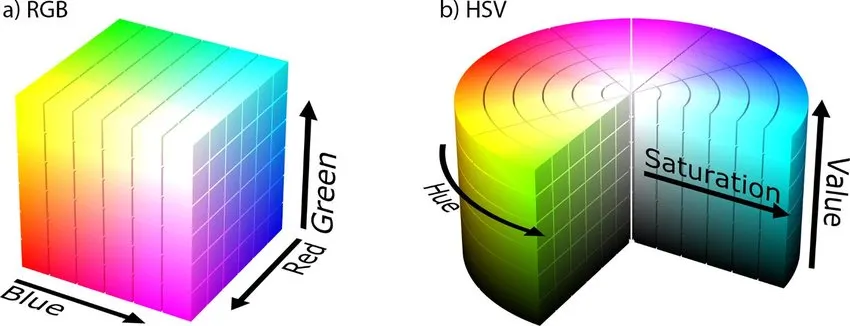
\includegraphics[width=0.72\linewidth]{figures/rgb_and_hsv.png}
\caption{Không gian màu RGB và HSV. HSV tách góc màu, cường độ màu và độ sáng,
giúp việc điều chỉnh sắc độ và độ bão hòa trực tiếp hơn.}
\label{fig:rgb-hsv}
\end{figure}

Quy trình đầy đủ gồm ba bước: chuyển RGB sang HSV, điều chỉnh $S$ hoặc $H$, sau
đó chuyển kết quả từ HSV về RGB.

\textbf{Chuyển RGB sang HSV.} Với các giá trị RGB đã được chuẩn hóa về $[0,1]$,
đặt $C_{\max}=\max(R,G,B)$, $C_{\min}=\min(R,G,B)$, và
$\Delta=C_{\max}-C_{\min}$. Khi đó
\begin{equation}
V=C_{\max}, \qquad
S =
\begin{cases}
0, & C_{\max}=0,\\
\Delta/C_{\max}, & C_{\max}>0.
\end{cases}
\label{eq:hsv-sv}
\end{equation}
Sắc độ được tính dựa trên kênh đạt giá trị $C_{\max}$:
\begin{equation}
H =
\begin{cases}
60^\circ\left(\frac{G-B}{\Delta}\bmod 6\right), & C_{\max}=R,\\
60^\circ\left(\frac{B-R}{\Delta}+2\right), & C_{\max}=G,\\
60^\circ\left(\frac{R-G}{\Delta}+4\right), & C_{\max}=B.
\end{cases}
\label{eq:hue}
\end{equation}
Khi $\Delta=0$, điểm ảnh không có hướng màu chủ đạo, do đó đặt $H=0$.

\textbf{Điều chỉnh độ bão hòa và sắc độ.}
Sau khi chuyển sang HSV, phép thay đổi độ bão hòa nhân $S$ với một hệ số và cắt
kết quả về $[0,1]$:
\begin{equation}
S' = \operatorname{clip}(kS,0,1).
\label{eq:saturation}
\end{equation}
Phép thay đổi sắc độ cộng thêm một góc và lấy phần dư theo vòng màu:
\begin{equation}
H' = (H+\Delta H) \bmod 360^\circ.
\label{eq:hue-shift}
\end{equation}

\textbf{Chuyển HSV về RGB.}
Giá trị HSV sau khi điều chỉnh được chuyển ngược về RGB. Đặt
$C=VS$, $X=C(1-|((H/60^\circ)\bmod 2)-1|)$, và $m=V-C$. Giá trị RGB tạm thời
$(R',G',B')$ được chọn theo vùng sắc độ:
\begin{equation}
(R',G',B') =
\begin{cases}
(C,X,0), & 0^\circ \le H < 60^\circ,\\
(X,C,0), & 60^\circ \le H < 120^\circ,\\
(0,C,X), & 120^\circ \le H < 180^\circ,\\
(0,X,C), & 180^\circ \le H < 240^\circ,\\
(X,0,C), & 240^\circ \le H < 300^\circ,\\
(C,0,X), & 300^\circ \le H < 360^\circ.
\end{cases}
\label{eq:hsv-rgb-sector}
\end{equation}
Giá trị RGB cuối cùng là $(R'+m,G'+m,B'+m)$, sau đó được đưa về miền $[0,255]$.

\subsubsection{Ảnh âm bản và hiệu chỉnh gamma}

Phép âm bản và hiệu chỉnh gamma đều giữ nguyên kích thước ảnh đầu vào. Phép âm
bản không có tham số và đảo ngược cường độ từng điểm ảnh:
\begin{equation}
I_{\text{out}} = 255 - I_{\text{in}}.
\label{eq:negative}
\end{equation}
Hiệu chỉnh gamma sử dụng tham số $\gamma$ và áp dụng một đường cong độ sáng phi
tuyến:
\begin{equation}
I_{\text{out}} = 255\left(\frac{I_{\text{in}}}{255}\right)^\gamma.
\label{eq:gamma}
\end{equation}
Giá trị $\gamma<1$ làm sáng các vùng tối, trong khi $\gamma>1$ làm ảnh tối hơn.

% =====================================================================
\section{Thiết lập thí nghiệm và độ đo đánh giá}
% =====================================================================

Các thí nghiệm sử dụng ảnh mẫu \texttt{lena.jpg} có kích thước
$1024 \times 680$ điểm ảnh và 3 kênh màu. Mỗi kết quả từ cài đặt thủ công bằng NumPy được so
sánh với kết quả tương ứng từ hàm của thư viện OpenCV. Việc đánh giá sử dụng bốn độ đo: thời gian
thực thi, mức sử dụng bộ nhớ, MAE và PSNR.

Thời gian thực thi cho biết một phép xử lý mất bao lâu để hoàn thành. Mức sử
dụng bộ nhớ cho biết lượng bộ nhớ đỉnh được cấp phát trong quá trình xử lý. Với
hai độ đo này, giá trị càng thấp thì kết quả càng tốt.

\textbf{Lưu ý.} Vì các hàm lõi của OpenCV được cài đặt và tối ưu bằng C/C++ nên thông tin bộ nhớ mà nhóm đo được từ phía Python có thể thấp hơn mức sử dụng thực tế của OpenCV.

MAE đo sự sai khác tuyệt đối trung bình giữa hai ảnh:
\begin{equation}
\operatorname{MAE}(A,B)=\frac{1}{N}\sum_{i=1}^{N}|A_i-B_i|.
\label{eq:mae}
\end{equation}
PSNR đo mức sai khác tương đối so với toàn miền cường độ 8-bit:
\begin{equation}
\operatorname{PSNR}(A,B)=10\log_{10}\left(\frac{255^2}{\operatorname{MSE}(A,B)}\right).
\label{eq:psnr}
\end{equation}
Nếu hai ảnh giống hệt nhau, MSE bằng 0 và PSNR được ghi nhận là \infpsnr.

Thông thường, các độ đo này cần được đọc cùng nhau để có được các thông tin hữu ích. Ví dụ, MAE thấp và PSNR cao cho thấy kết quả của cách thủ
công rất gần với OpenCV. MAE bằng 0 và PSNR vô hạn nghĩa là hai kết quả khớp nhau hoàn toàn. Trong khi đó, thời gian và bộ nhớ thể hiện chi phí và độ hiệu quả trong cách cài đặt của nhóm.

% =====================================================================
\section{Kết quả}
% =====================================================================

\subsection{Đọc và hiển thị ảnh}

Hình~\ref{fig:io} cho thấy ảnh được đọc bằng OpenCV và hiển thị bằng
Matplotlib. Nhãn phía dưới ảnh thể hiện chiều rộng, chiều cao và số kênh màu.

\begin{figure}[H]
\centering
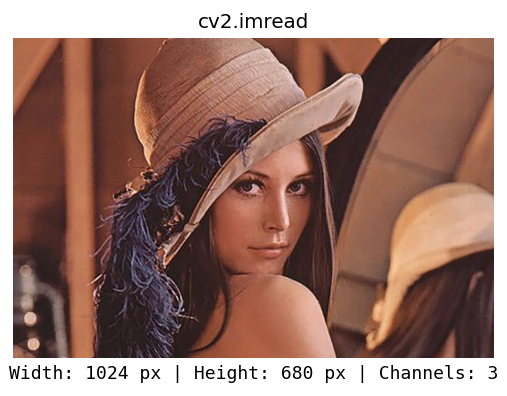
\includegraphics[width=0.5\linewidth]{figures/01_io.png}
\caption{Ảnh được đọc bằng OpenCV và hiển thị bằng Matplotlib. Thông tin chiều
rộng, chiều cao và số kênh màu được hiển thị phía dưới ảnh.}
\label{fig:io}
\end{figure}

\subsection{Thay đổi kích thước và xoay ảnh}

Hình~\ref{fig:resize} và Hình~\ref{fig:rotate} so sánh kết quả thủ công với
OpenCV cho các phép biến đổi hình học. Kết quả định lượng được trình bày trong
Bảng~\ref{tab:resize-results} và~\ref{tab:rotate-results}. Hai phép thay đổi
kích thước có MAE rất nhỏ và PSNR cao vì ánh xạ tọa độ thủ công tuân theo quy
ước tâm điểm ảnh của OpenCV. Phép xoay $30^\circ$ có sai khác lớn hơn nhưng vẫn
nhỏ, chủ yếu do khác biệt trong nội suy và làm tròn. Phép xoay $90^\circ$ khớp
chính xác và cách cài đặt thủ công cũng nhanh hơn đáng kể vì đây là trường hợp đặc biệt, ta có thể thực hiện bằng chuyển vị ma trận kết hợp với lật ảnh.

\begin{figure}[H]
\centering
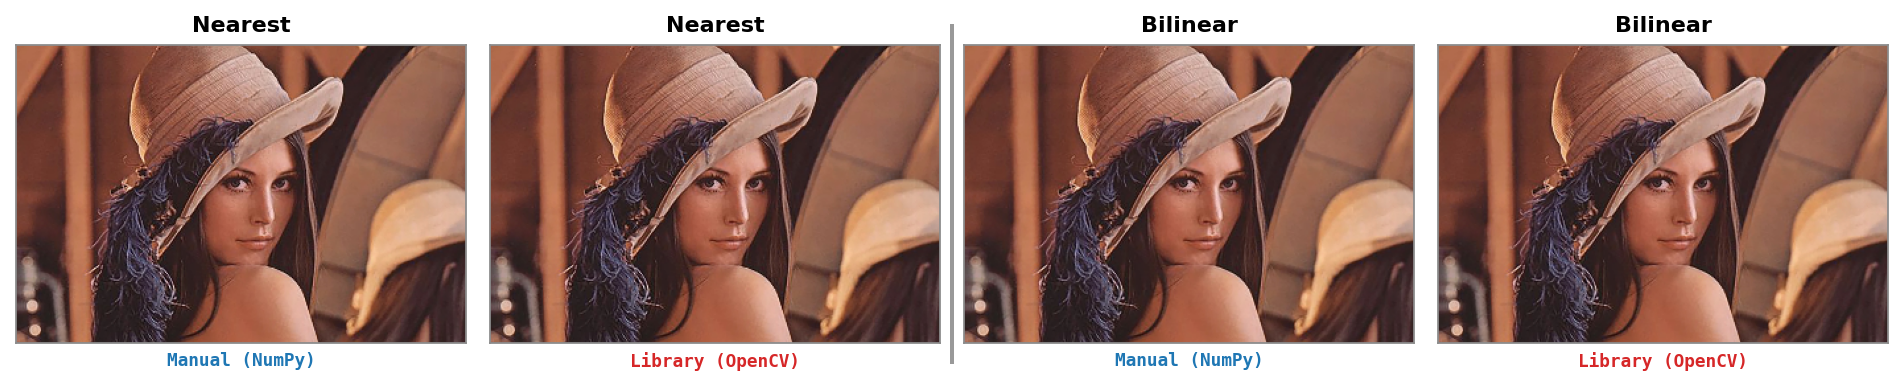
\includegraphics[width=\linewidth]{figures/02_resize.png}
\caption{Kết quả thay đổi kích thước. Mỗi phép xử lý được hiển thị thành một
cặp: NumPy thủ công bên trái và OpenCV bên phải.}
\label{fig:resize}
\end{figure}

\begin{table}[H]
\centering
\caption{Thời gian, bộ nhớ và chất lượng của phép thay đổi kích thước trên
\texttt{lena.jpg}.}
\label{tab:resize-results}
\begin{adjustbox}{max width=\linewidth}
\begin{tabular}{lrrrrrr}
\toprule
\textbf{Phép xử lý} &
\shortstack{\textbf{Thời gian NumPy}\\\textbf{(ms)}} &
\shortstack{\textbf{Thời gian OpenCV}\\\textbf{(ms)}} &
\shortstack{\textbf{Bộ nhớ NumPy}\\\textbf{(KiB)}} &
\shortstack{\textbf{Bộ nhớ OpenCV}\\\textbf{(KiB)}} &
\textbf{MAE} &
\shortstack{\textbf{PSNR}\\\textbf{(dB)}} \\
\midrule
resize lân cận gần nhất & 1.721791 & 0.762833 & 362.294922   & 225.873047  & 0.010878 & 56.133817 \\
resize song tuyến tính  & 9.585458 & 0.404208 & 20824.558594 & 225.873047  & 0.004745 & 71.368578 \\
\bottomrule
\end{tabular}
\end{adjustbox}
\end{table}

\begin{figure}[H]
\centering
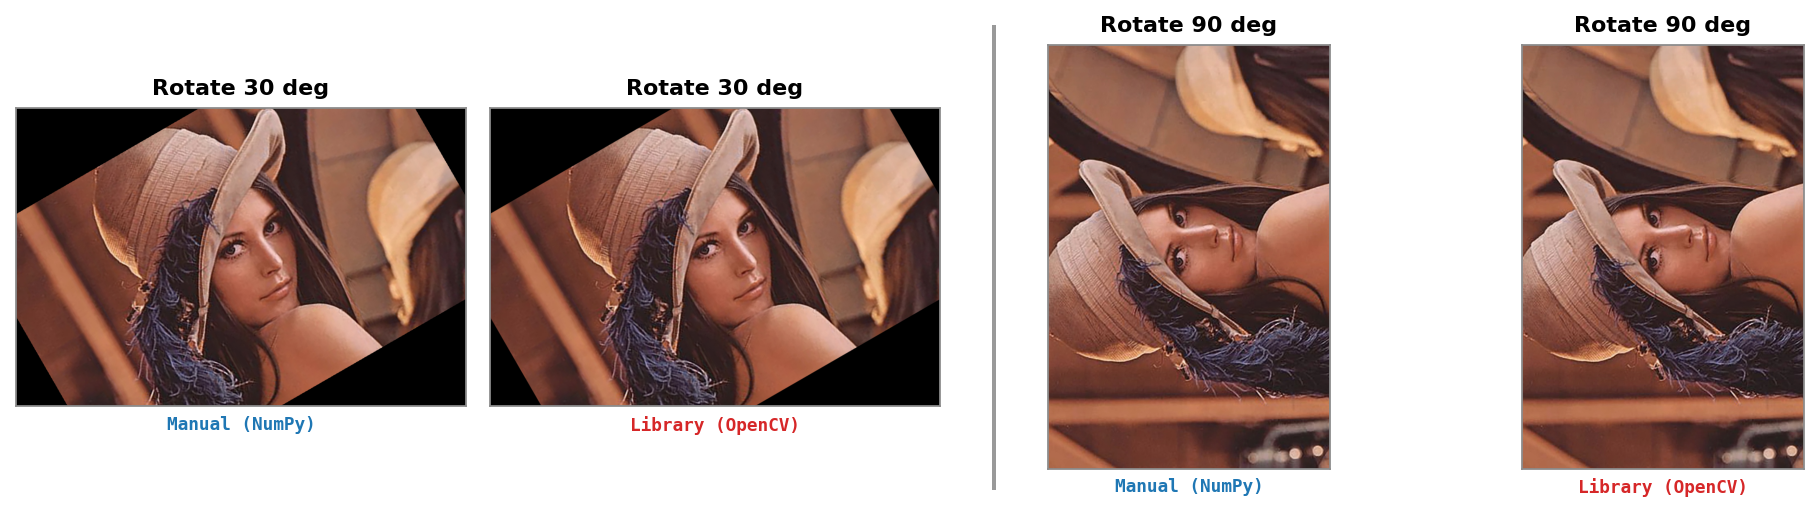
\includegraphics[width=\linewidth]{figures/03_rotate.png}
\caption{Kết quả xoay ảnh với góc $30^\circ$ và $90^\circ$. Trường hợp góc bất
kỳ dùng nội suy song tuyến tính; trường hợp $90^\circ$ là chính xác.}
\label{fig:rotate}
\end{figure}

\begin{table}[H]
\centering
\caption{Thời gian, bộ nhớ và chất lượng của phép xoay ảnh trên
\texttt{lena.jpg}.}
\label{tab:rotate-results}
\begin{adjustbox}{max width=\linewidth}
\begin{tabular}{lrrrrrr}
\toprule
\textbf{Phép xử lý} &
\shortstack{\textbf{Thời gian NumPy}\\\textbf{(ms)}} &
\shortstack{\textbf{Thời gian OpenCV}\\\textbf{(ms)}} &
\shortstack{\textbf{Bộ nhớ NumPy}\\\textbf{(KiB)}} &
\shortstack{\textbf{Bộ nhớ OpenCV}\\\textbf{(KiB)}} &
\textbf{MAE} &
\shortstack{\textbf{PSNR}\\\textbf{(dB)}} \\
\midrule
xoay 30 độ & 117.704917 & 0.588708 & 193806.064453 & 2040.296875 & 0.138756 & 38.837706 \\
xoay 90 độ                 & 0.011875   & 0.606250 & 0.226562      & 2040.250000 & 0.000000 & \infpsnr \\
\bottomrule
\end{tabular}
\end{adjustbox}
\end{table}

\subsection{Độ sáng và độ tương phản}

Hình~\ref{fig:brightness-contrast} minh họa cả hai trường hợp tăng/giảm độ sáng
và tăng/giảm độ tương phản. Bảng~\ref{tab:bc-results} cho thấy độ sáng và độ
tương phản khớp chính xác với OpenCV khi dùng phép tính bão hòa (MAE bằng 0
và PSNR là \infpsnr).

\begin{figure}[H]
\centering
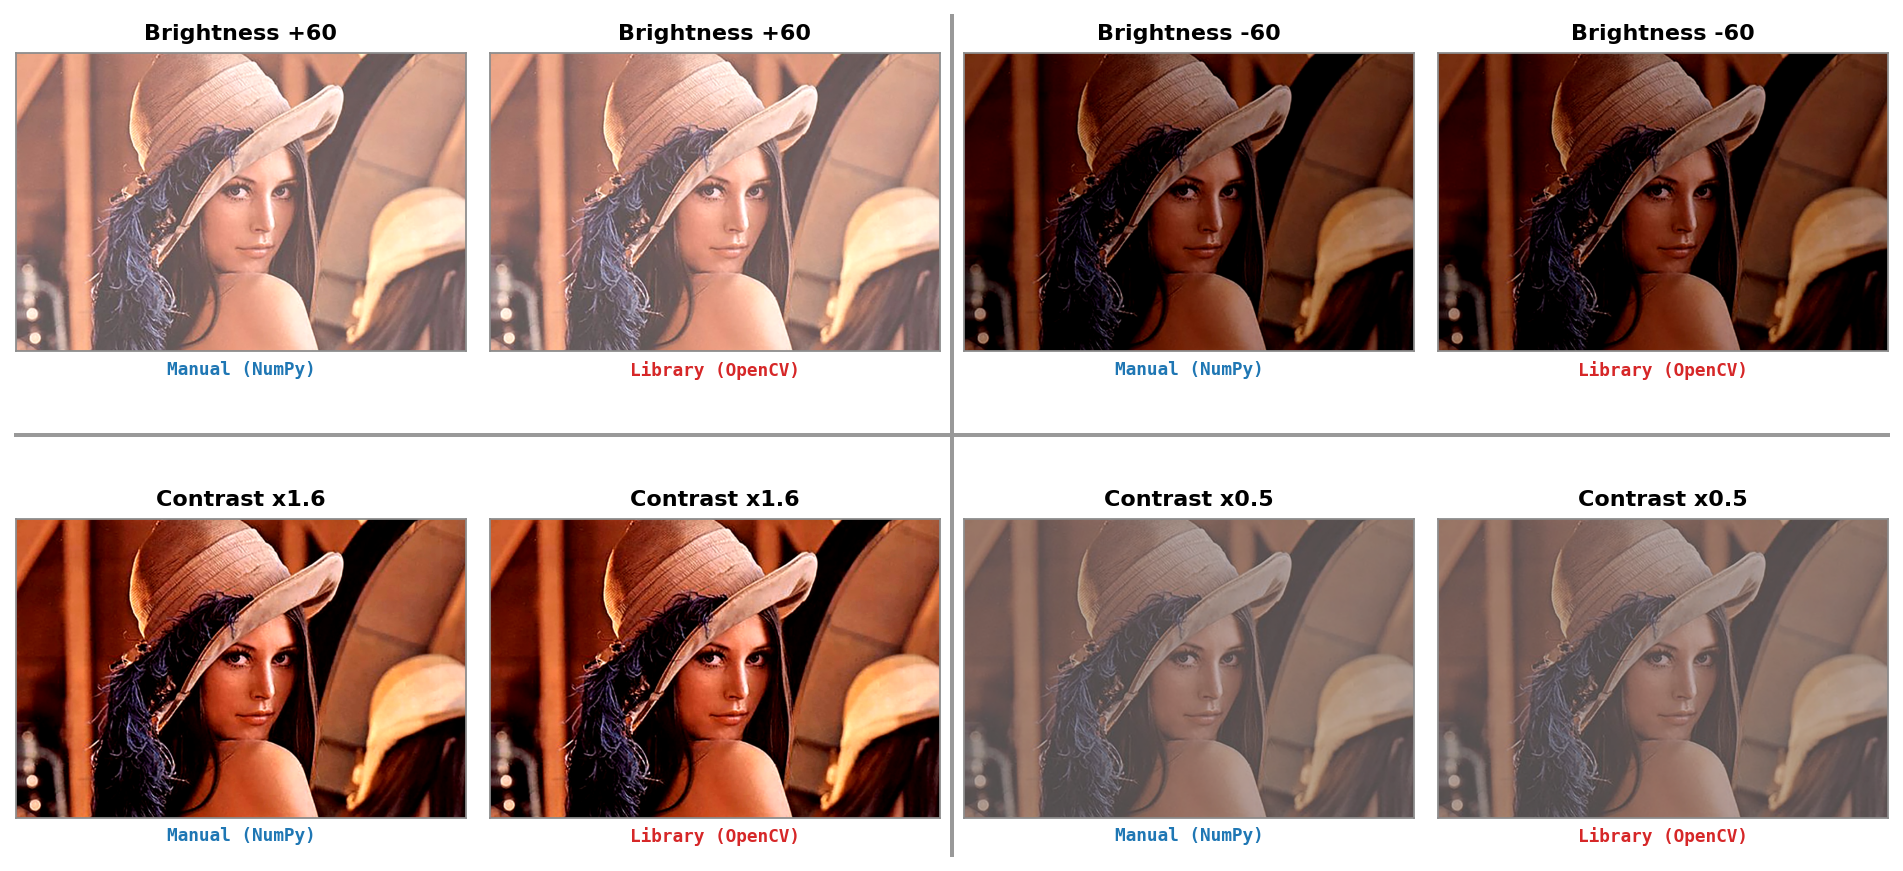
\includegraphics[width=\linewidth]{figures/04_brightness_contrast.png}
\caption{Các phép biến đổi độ sáng và độ tương phản. Hình bao gồm cả ví dụ tăng
và giảm cho mỗi phép biến đổi.}
\label{fig:brightness-contrast}
\end{figure}

\begin{table}[H]
\centering
\caption{Thời gian, bộ nhớ và chất lượng của phép thay đổi độ sáng và độ tương
phản trên \texttt{lena.jpg}.}
\label{tab:bc-results}
\begin{adjustbox}{max width=\linewidth}
\begin{tabular}{lrrrrrr}
\toprule
\textbf{Phép xử lý} &
\shortstack{\textbf{Thời gian NumPy}\\\textbf{(ms)}} &
\shortstack{\textbf{Thời gian OpenCV}\\\textbf{(ms)}} &
\shortstack{\textbf{Bộ nhớ NumPy}\\\textbf{(KiB)}} &
\shortstack{\textbf{Bộ nhớ OpenCV}\\\textbf{(KiB)}} &
\textbf{MAE} &
\shortstack{\textbf{PSNR}\\\textbf{(dB)}} \\
\midrule
độ sáng +60      & 1.589333  & 0.536542 & 12241.472656 & 4080.187500 & 0.000000 & \infpsnr \\
độ tương phản x1.6 & 10.735709 & 0.546042 & 24480.851562 & 4080.187500 & 0.000000 & \infpsnr \\
\bottomrule
\end{tabular}
\end{adjustbox}
\end{table}

\subsection{Biến đổi màu}

Hình~\ref{fig:color-results} trình bày các phép chuyển ảnh xám, âm bản, gamma,
độ bão hòa và sắc độ. Bảng~\ref{tab:color-results} cho thấy ảnh âm bản và gamma
khớp chính xác; chuyển ảnh xám chỉ có sai khác làm tròn rất nhỏ. Độ bão hòa và
sắc độ nhìn trực quan rất gần nhau nhưng MAE khác 0, vì OpenCV lưu HSV ở dạng số
nguyên với kênh hue được lượng tử về $[0,179]$, trong khi cài đặt thủ công dùng
HSV dạng số thực với hue tính theo độ.

\begin{figure}[H]
\centering
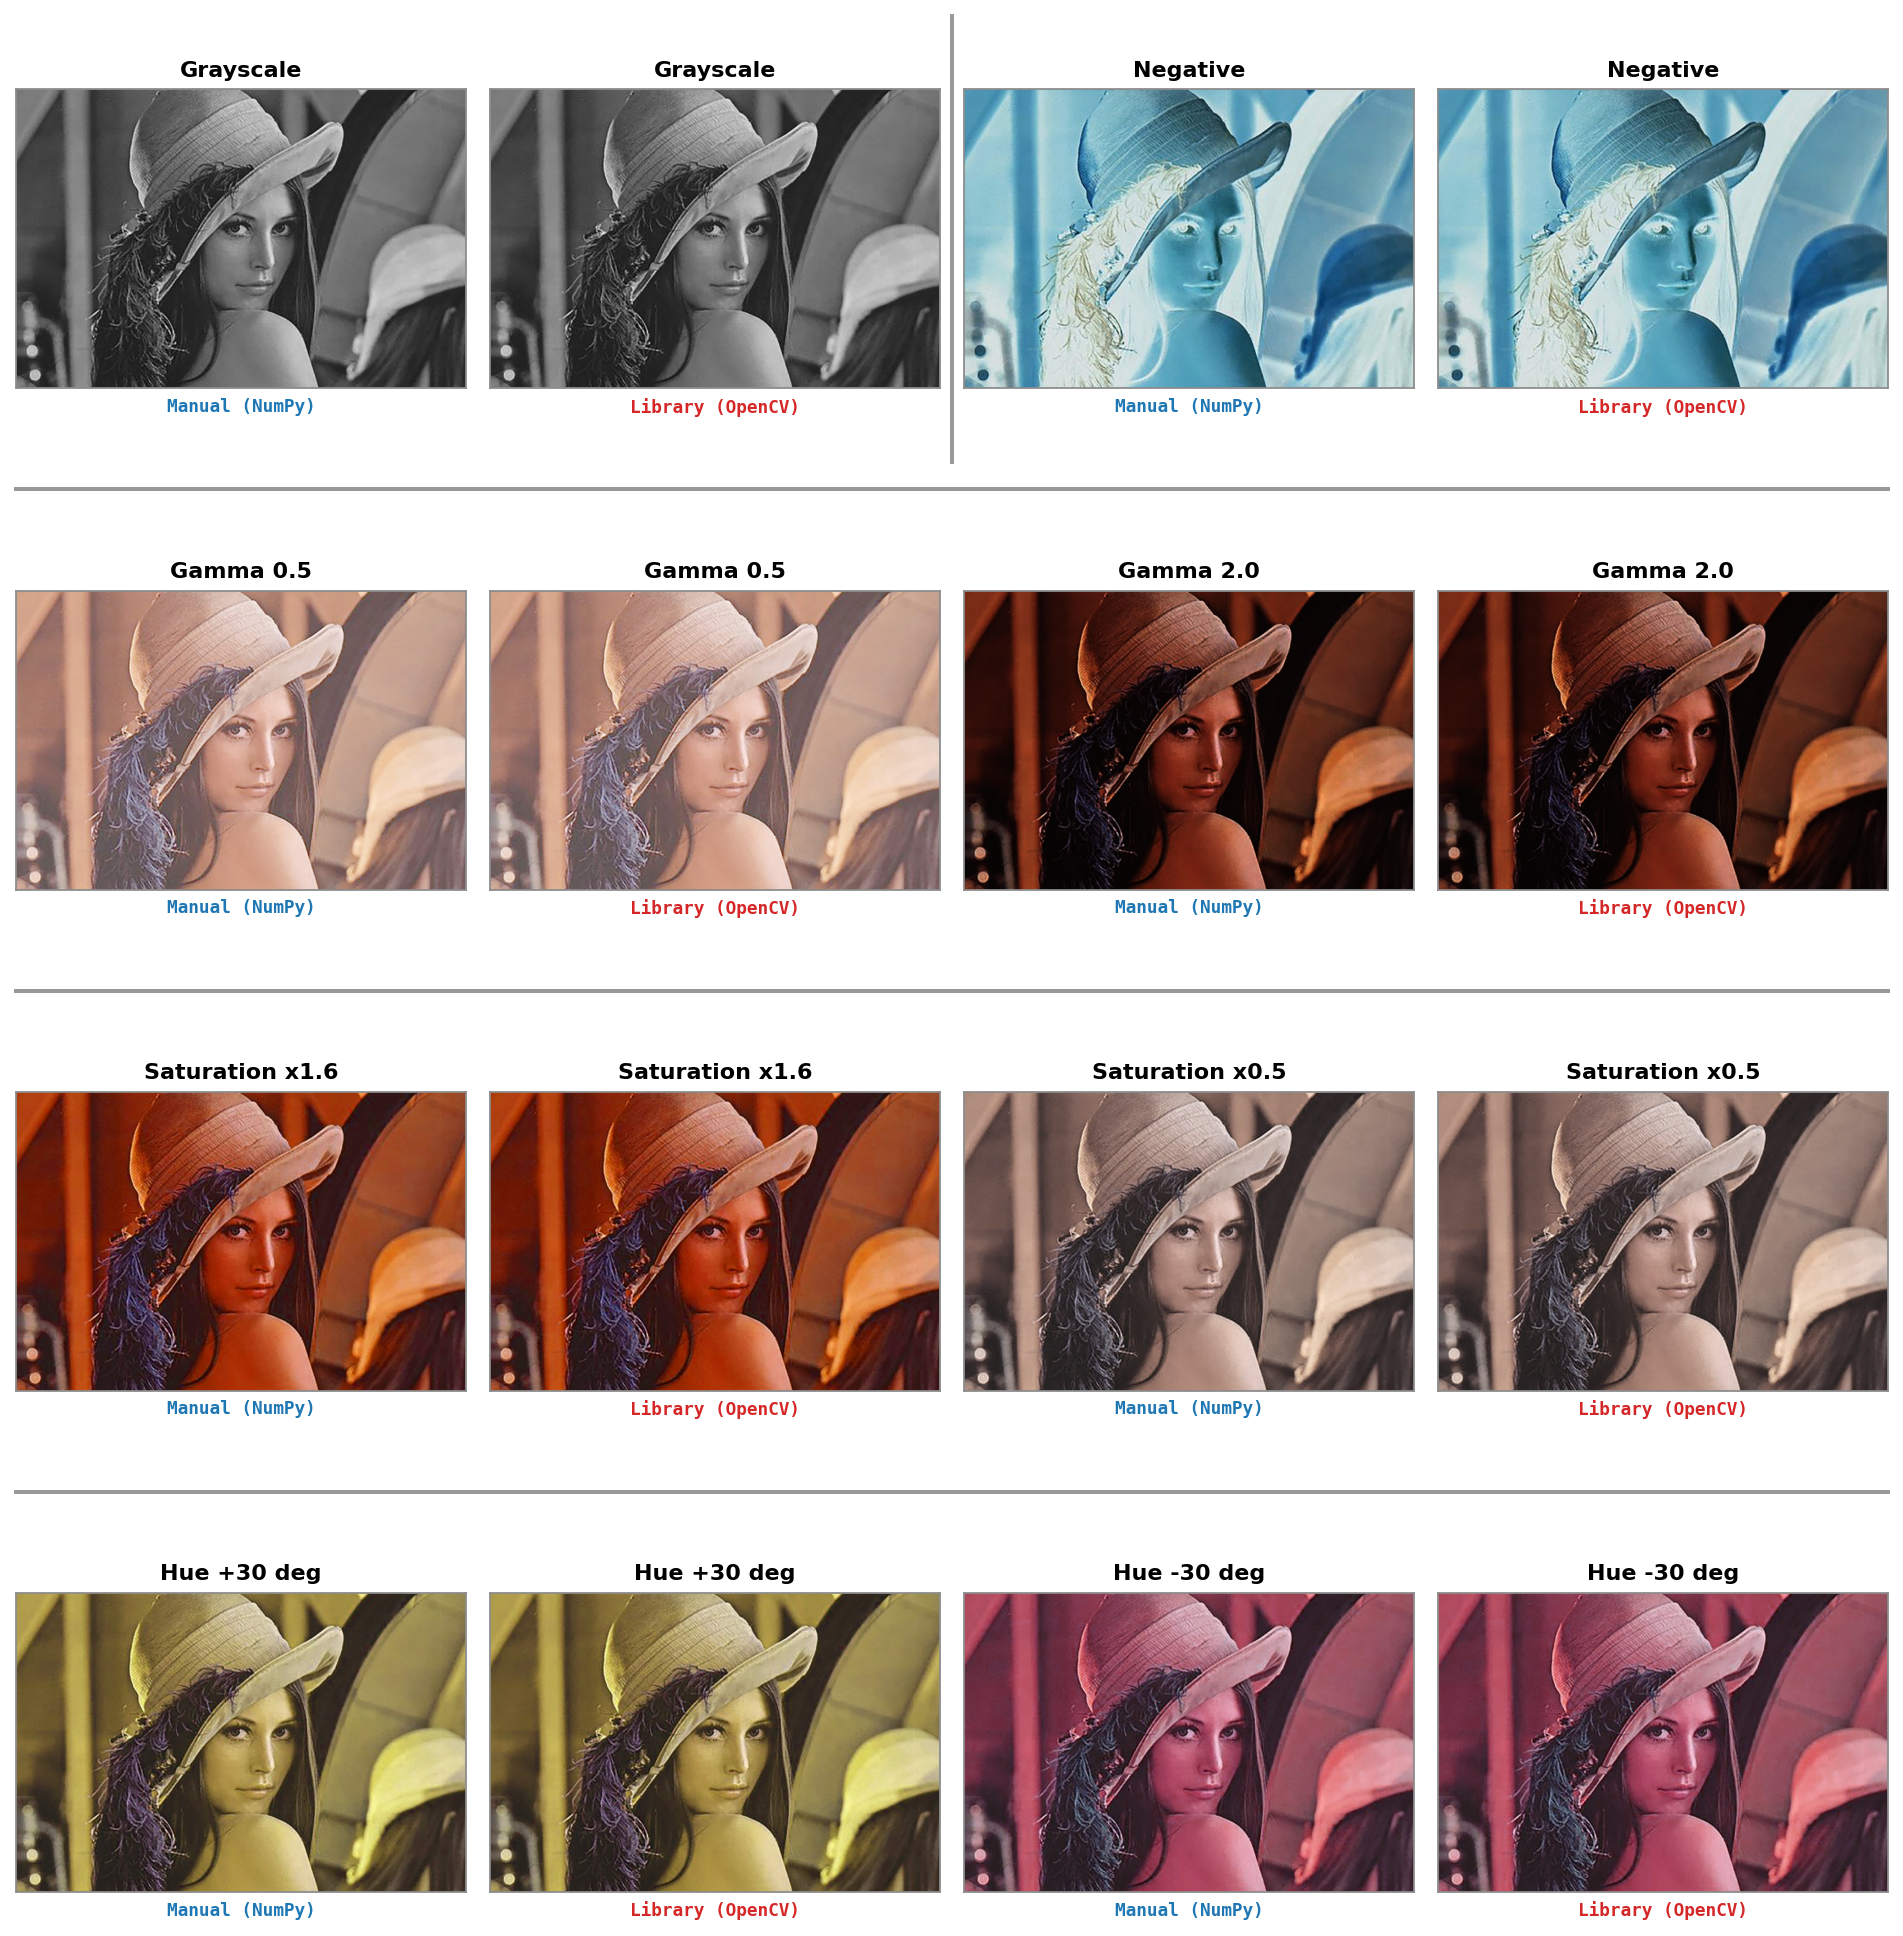
\includegraphics[width=\linewidth]{figures/05_color.png}
\caption{Kết quả các phép biến đổi màu. Hình bao gồm ảnh xám, âm bản, gamma nhỏ
hơn và lớn hơn một, tăng/giảm độ bão hòa, và dịch sắc độ theo hai chiều.}
\label{fig:color-results}
\end{figure}

\begin{table}[H]
\centering
\caption{Thời gian, bộ nhớ và chất lượng của các phép biến đổi màu trên
\texttt{lena.jpg}.}
\label{tab:color-results}
\begin{adjustbox}{max width=\linewidth}
\begin{tabular}{lrrrrrr}
\toprule
\textbf{Phép xử lý} &
\shortstack{\textbf{Thời gian NumPy}\\\textbf{(ms)}} &
\shortstack{\textbf{Thời gian OpenCV}\\\textbf{(ms)}} &
\shortstack{\textbf{Bộ nhớ NumPy}\\\textbf{(KiB)}} &
\shortstack{\textbf{Bộ nhớ OpenCV}\\\textbf{(KiB)}} &
\textbf{MAE} &
\shortstack{\textbf{PSNR}\\\textbf{(dB)}} \\
\midrule
ảnh xám          & 4.476833  & 0.068250 & 16321.281250 & 680.093750   & 0.000003 & 103.548592 \\
độ bão hòa x1.6  & 44.441375 & 3.141875 & 66646.609375 & 12920.914062 & 0.455611 & 50.069759 \\
sắc độ +30 độ    & 43.972500 & 1.885375 & 66643.140625 & 4760.681641  & 0.400402 & 51.361964 \\
âm bản           & 5.798667  & 0.166708 & 24480.851562 & 2040.093750  & 0.000000 & \infpsnr \\
gamma 0.5        & 7.193083  & 0.230334 & 24480.898438 & 2041.554688  & 0.000000 & \infpsnr \\
\bottomrule
\end{tabular}
\end{adjustbox}
\end{table}

% =====================================================================
\section{Thảo luận}
% =====================================================================

\runin{Chất lượng ảnh đầu ra.} Một số phép xử lý mà nhóm cài đặt thủ công có độ khớp chính xác với OpenCV, gồm điều chỉnh độ sáng,
độ tương phản, âm bản, gamma và xoay $90^\circ$. Phép thay đổi kích thước ảnh và xoay ảnh đạt được kết quả rất gần với OpenCV nhưng không hoàn toàn giống nhau do khác biệt về cách cài đặt nội suy và các phép làm tròn số. Với độ bão hòa và sắc độ, sai khác chủ yếu của nhóm đến từ việc OpenCV sử dụng cách biểu diễn
HSV lượng tử.

\runin{Thời gian chạy và bộ nhớ.} OpenCV nhanh hơn đáng kể trong hầu hết các phép xử
lý vì các hàm lõi của thư viện này được tối ưu bằng C/C++, hạn chế các biến trung gian, tận dụng truy
cập bộ nhớ hiệu quả và có thể dùng SIMD hoặc đa luồng. Cài đặt thủ công bằng NumPy của nhóm tuy dễ đọc và
đã có tính vector hóa nhưng vẫn có nhiều biểu thức tạo ra các mảng trung gian kích thước lớn. Điều này thể hiện rõ nhất ở phép xoay ảnh.

% =====================================================================
\section{Kết luận}
% =====================================================================

Bài thực hành cho thấy NumPy rất hữu ích để biểu diễn và hiểu các thuật toán
đằng sau những phép xử lý ảnh phổ biến. Tuy nhiên, OpenCV vẫn nhanh hơn và hiệu
quả bộ nhớ hơn nhiều trong các trường hợp sử dụng thực tế. Các phép toán cài đặt thủ công của nhóm
đạt độ chính xác tốt: nhiều phép xử lý khớp hoàn toàn với OpenCV, còn các sai
khác còn lại đều nhỏ và có thể giải thích được nguồn gốc xuất phát từ các phép tính nội suy, làm tròn hoặc lượng tử
hóa HSV. Vì vậy, phần so thực hành này vừa chúng em giúp hiểu rõ thuật toán và hiểu rõ lý do
các thư viện xử lý ảnh tối ưu như OpenCV thường được ưu tiên trong ứng dụng thực tế.

% =====================================================================
\section{Tự đánh giá và bảng phân công công việc}
% =====================================================================

Bảng~\ref{tab:completion} tóm tắt mức độ hoàn thành các yêu cầu chính của bài
thực hành. Nhóm đã \textbf{hoàn thành đầy đủ} các phần cài đặt thủ công bằng NumPy, phần
đối chiếu với OpenCV, phần sinh hình minh họa và phần đánh giá định lượng bằng
thời gian, bộ nhớ, MAE và PSNR.
Bảng~\ref{tab:members} trình bày phân công công việc theo thành viên trong nhóm.


\begin{table}[H]
\centering
\caption{Tự đánh giá mức độ hoàn thành các yêu cầu.}
\label{tab:completion}
\begin{adjustbox}{max width=\linewidth}
\begin{tabular}{c p{8.2cm} c c}
\toprule
\textbf{STT} & \textbf{Yêu cầu} & \textbf{NumPy thủ công} & \textbf{OpenCV/Thư viện} \\
\midrule
1 & Đọc và hiển thị ảnh bằng OpenCV và Matplotlib & -- & \checkmark\,(100\%) \\
2 & Thay đổi kích thước bằng nội suy lân cận gần nhất và song tuyến tính & \checkmark\,(100\%) & \checkmark\,(100\%) \\
3 & Xoay ảnh góc bất kỳ và xoay $90^\circ$ & \checkmark\,(100\%) & \checkmark\,(100\%) \\
4 & Điều chỉnh độ sáng và độ tương phản & \checkmark\,(100\%) & \checkmark\,(100\%) \\
5 & Chuyển ảnh xám, âm bản và hiệu chỉnh gamma & \checkmark\,(100\%) & \checkmark\,(100\%) \\
6 & Điều chỉnh độ bão hòa và sắc độ thông qua không gian màu HSV & \checkmark\,(100\%) & \checkmark\,(100\%) \\
7 & So sánh định lượng bằng thời gian, bộ nhớ, MAE và PSNR & \multicolumn{2}{c}{\checkmark\,(100\%)} \\
8 & Tạo hình kết quả phục vụ báo cáo và bảng tổng hợp số liệu & \multicolumn{2}{c}{\checkmark\,(100\%)} \\
\bottomrule
\end{tabular}
\end{adjustbox}
\end{table}

\begin{table}[H]
\centering
\caption{Phân công công việc và tỷ lệ đóng góp của thành viên.}
\label{tab:members}
\begin{adjustbox}{max width=\linewidth}
\begin{tabular}{c l c p{7.2cm} c}
\toprule
\textbf{STT} & \textbf{Họ và tên} & \textbf{Mã học viên} & \textbf{Công việc chính} & \textbf{Đóng góp} \\
\midrule
1 & Lưu Thị Yến Nhi & 25C11014 &
  Đọc/hiển thị ảnh; Cài đặt resize và xoay ảnh; Hỗ trợ kiểm tra kết quả so sánh; Viết báo cáo. & 50\% \\
2 & Hoàng Trọng Vũ & 25C15028 &
  Cài đặt biến đổi độ sáng, độ tương phản và màu sắc; So sánh với OpenCV; Viết báo cáo & 50\% \\
\midrule
\multicolumn{4}{r}{\textbf{Tổng cộng}} & \textbf{100\%} \\
\bottomrule
\end{tabular}
\end{adjustbox}
\end{table}


\bibliographystyle{plain}
\bibliography{references}

\end{document}
